\documentclass{article}

\usepackage{fullpage}
\usepackage{url}
\usepackage{graphicx}
\usepackage{amsmath}
\usepackage{physics}
\usepackage{mathtools}
\usepackage{bbold}

\DeclareMathOperator{\erfi}{erfi}
\newcommand{\R}{\ensuremath{\mathbb{R}}}
\newcommand{\C}{\ensuremath{\mathbb{C}}}

\title{Quantum Mechanics I Excercise 7}
\author{Idan Stark}
\date{\today}

\begin{document}
\maketitle

\section{The emission of radiation by a particle in isotropic harmonic potential}
We consider in this section the emission of radiation by a particle in isotropic harmonic potential. The particle will have charge $q$, and thus the matter hamiltonian can be written as
\begin{equation}
    H_{matter} = \frac{\boldsymbol{p}^2}{2m} + \frac{1}{2}m\omega^2\boldsymbol{r}^2
\end{equation}
The corresponding states are defined by the three quantum numbers $n$ for the energy level, and $(l, m)$ for the angular momentum:
\begin{equation}
    \ket{klm} = \frac{1}{r}u_{k, l}(r) Y^{m}_l(\theta, \varphi)
\end{equation}
Where $Y^{m}_l$ are the spherical harmonics and $u_{k,l}$ are the solution to the radial equation
\begin{equation}
    \left[\frac{d^2}{dr^2} - \beta^4r^2 - \frac{l(l+1)}{r^2} + \varepsilon_{k, l}\right]u_{k,l}(r) = 0
\end{equation}
and the total energy is
\begin{equation}
    E_{klm} = \hbar \omega \left(k + l +\frac{3}{2}\right) \equiv \hbar \omega \left(n + \frac{3}{2} \right)
\end{equation}
Last thing to notice is that since $u_{k,l}$ have parity $l+1$, the total radial part of $\ket{klm}$ has parity $l$.
\subsection{The emission rate}
The emission rate follows Fermi's golden rule:
\begin{equation}
    \Gamma_{i \rightarrow f} = \frac{2\pi}{\hbar}\left|\bra{f} V \ket{i}\right|^2\delta(E_i - E_f - \hbar \omega_k)
\end{equation}
Igonring spin, the interaction $V$ comes from the spatial matter-EM interraction $H_{I1}$, which can be written in terms of the possible photon wave numbers $\boldsymbol{k}_\alpha$:
\begin{equation}
    H_{I1} = \sum_{\boldsymbol{k}_{\alpha}}
    \left(\frac{\hbar}{2\epsilon_0\omega_k\Omega}\right)^{1/2}
    \left(\boldsymbol{j}_{-\boldsymbol{k}}\cdot\boldsymbol{\lambda}_{\boldsymbol{k}_\alpha}\right)
    \left(a_{\boldsymbol{k}_\alpha} + a^\dagger_{-\boldsymbol{k}_\alpha}\right)
\end{equation}
So, starting from some state $\ket{klm}$ of the harmonic oscillator and some without any photons $\ket{\{0_{\boldsymbol{k}_\alpha}\}}$, and ending with a different state of the harmonic oscillator $\ket{k'l'm'}$ and a single photon $\ket{1_{\boldsymbol{k}_\alpha}, \{0_{\boldsymbol{k}'_{\alpha'}}\}}$, each operator in the interaction acts upon it's part of the state (the current operator acts on the harmonic oscillator while the potential operator acts on photons), resulting in the same result as we saw in class:
\begin{equation}
\begin{gathered}
    \bra{f} H_{I1} \ket{i} = 
    \sum_{\boldsymbol{k}''_{\alpha''}}
    \left(\frac{\hbar}{2\epsilon_0\omega_k\Omega}\right)^{1/2}
    \bra{k'l'm'}\boldsymbol{j}_{\boldsymbol{k''}_{\alpha''}}\cdot\boldsymbol{\lambda}_{\boldsymbol{k}''_{\alpha''}}\ket{klm}
    \bra{1_{\boldsymbol{k}_\alpha}, \{0_{\boldsymbol{k}'_{\alpha'}}\}}
        a_{\boldsymbol{k}''_{\alpha''}}e^{i\boldsymbol{k}\cdot\boldsymbol{r}}
        +
        a^\dagger_{\boldsymbol{k}''_{\alpha''}}e^{-i\boldsymbol{k}\cdot\boldsymbol{r}}
    \ket{\{0_{\boldsymbol{k}_\alpha}\}}
    = \\ =
    \left(\frac{\hbar}{2\epsilon_0\omega_k\Omega}\right)^{1/2}
    \bra{k'l'm'}\boldsymbol{j}_{\boldsymbol{k}}\cdot{\lambda}_{\boldsymbol{k}_{\alpha}}\ket{klm}
\end{gathered}
\end{equation}
Remembering that
\begin{equation}
    \boldsymbol{j}_{\boldsymbol{k}} = \frac{q}{2m}\left[
        \boldsymbol{p}e^{-i\boldsymbol{k}\cdot\boldsymbol{r}}
        + 
        e^{-i\boldsymbol{k}\cdot\boldsymbol{r}}\boldsymbol{p}
    \right]
\end{equation}
We can write:
\begin{equation}
\begin{gathered}
\label{eq:pre-lwa}
    \bra{f} H_{I1} \ket{i} = \left(\frac{\hbar}{2\epsilon_0\omega_k\Omega}\right)^{1/2}
    \frac{q}{2m}
    \left(
        \bra{k'l'm'}\boldsymbol{p}\cdot{\lambda}_{\boldsymbol{k}_{\alpha}}e^{-i\boldsymbol{k}\cdot\boldsymbol{r}}\ket{klm}
        +
        \bra{k'l'm'}e^{-i\boldsymbol{k}\cdot\boldsymbol{r}}\boldsymbol{p}\cdot{\lambda}_{\boldsymbol{k}_{\alpha}}\ket{klm}
    \right)
    = \\ = -\left(\frac{\hbar}{2\epsilon_0\omega_k\Omega}\right)^{1/2}
    \frac{qh^2}{2m}
    \int
    u_{n, l'}(r) Y^{m'*}_{l'}(\theta, \varphi)
    \left(
        \boldsymbol{\nabla}e^{-i\boldsymbol{k}\cdot\boldsymbol{r}}
    +
    e^{-i\boldsymbol{k}\cdot\boldsymbol{r}}\boldsymbol{\nabla}
    \right)\cdot{\lambda}_{\boldsymbol{k}_{\alpha}} u_{k, l}(r) Y^{m}_{l}(\theta, \varphi)
    \sin\theta dr d\theta d\varphi
\end{gathered}
\end{equation}

\subsection{The Long Wavelength Apprxoimation}
The Long Wavelength Apprxoimation will hold if the photon wavelength $\lambda$ is much larger then the typical size of the emitting system. In this case, the typical size comes from the mass $m$ and angular frequency $\omega$. From units considerations, we can see that the typical length is:
\begin{equation}
    L \sim \sqrt{\frac{\hbar}{\omega m}}
\end{equation}
The wavelength of the mitted photon is related to the energy levels of the harmonic oscillator using conservation of energy. They thus have the same angular frequency, and the requirement for the LWA $L \ll \lambda$ can be written as:
\begin{equation}
    \frac{\hbar}{\omega m} \ll \lambda^2 = \frac{4\pi^2 c^2}{\omega^2}
\end{equation}
or
\begin{equation}
    mc^2 \gg \hbar\omega
\end{equation}
In other words, the rest mass of the oscillator must be much higher then its energy levels, which is the basic requirement for working in a non-reletavistic paradigm.

\subsection{The dipole transition}
To use the LWA, it will be useful to work in Fock space, starting from equation \ref{eq:pre-lwa} and building up using creation and anhilation operators for the harmonic oscillator. From LWA, we can write the exponent in equation \ref{eq:pre-lwa} as a series of powers, starting from the zeroth order, corresponding to the dipole transition.
\newline
In zeroth order, $H_{I1}$ then has only the creation an annihilation operators from $\boldsymbol{p} \propto a^\dagger + a$, which is a single creation / annihilation in each cartesian direction.
\newline
In the angular direction, the selection rules are identical to those of any isotropic system with radial parity equals to $l$, (since they all have the same dependency on the spherical harmonics in their wave function) including the hydrogen atom as we saw in class:
\begin{equation}
    \Delta l = \pm 1
    \qquad
    \Delta m = 0, \pm 1
\end{equation}
The radial result is that the total energy quantum number $n$ can change by a total of $\Delta n = \pm 1$, exciting one of the axis. This works well with the fact that in the solutions to the 3D isotropic harmonic oscillator, $l$ is only allowed to have the same parity as $n$:
\begin{equation}
    \Delta n = \pm 1
\end{equation}
Some examples (writing in $\ket{nlm}$) include $\ket{110}\rightarrow\ket{000}$, $\ket{222}\rightarrow\ket{111}$, $\ket{221}\rightarrow\ket{110}$.
These selection rules can be seen in figure \ref{fig:energy-levels}.
\begin{figure}[h]
    \centering
    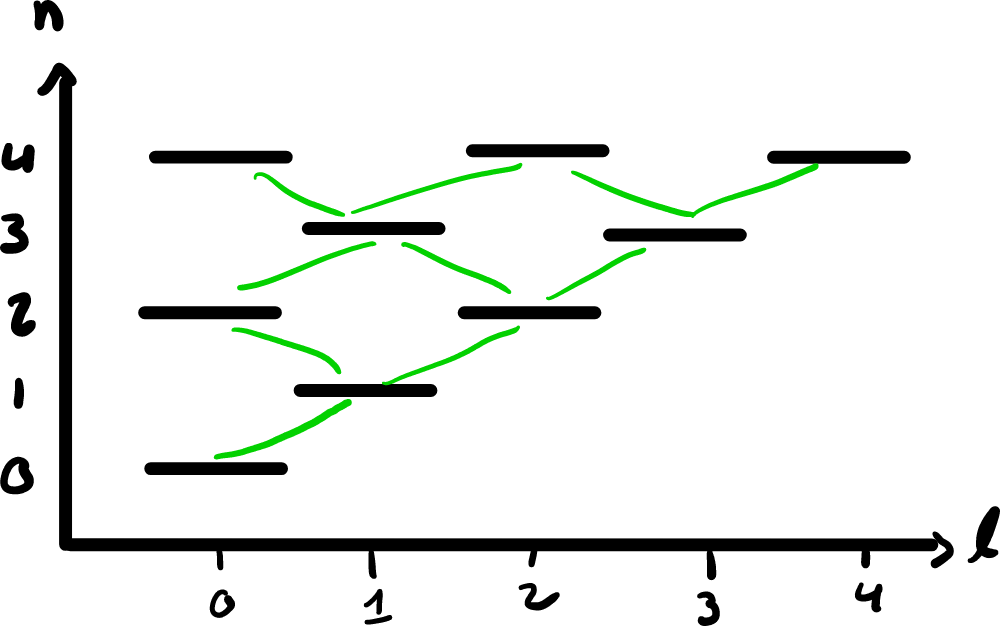
\includegraphics[width=0.6\textwidth]{Notewise-Character Sheet v0.5a-20260327162934.png}
    \caption{Energy levels of the 3D istropic harmonic oscilator (black) and the electric dipole transitions between them (green)}
    \label{fig:energy-levels}
\end{figure}
\subsection{Angualr Distribution and polarization of the $\ket{11m}\rightarrow\ket{000}$ transition}
As we saw in class, the angualr distribution can be written as:
\begin{equation}
    \frac{dN_{\boldsymbol{k}_\alpha}}{d\gamma} = \frac{\omega}{8\pi^2c^3\epsilon_0\hbar}\left|\bra{n'l'm'}\boldsymbol{j}_{\boldsymbol{k}}\cdot{\lambda}_{\boldsymbol{k}_{\alpha}}\ket{nlm}\right|^2
\end{equation}
Let us calcualte then the matrix element using the dipole apprxoimation. Writing the dipole operator $
\boldsymbol{d} = e\boldsymbol{r}$ in the basis of sperical harmonics:
\begin{equation}
    d_\mu = q\sqrt{\frac{4\pi}{3}} r Y^{\mu}_1(\theta, \varphi)
\end{equation}
We find the matrix element to be
\begin{equation}
\begin{gathered}
    \bra{000}\boldsymbol{j}_{\boldsymbol{k}}\cdot{\lambda}_{\boldsymbol{k}_{\alpha}}\ket{11m} \approx
    {\lambda}_{\boldsymbol{k}_{\alpha}}\cdot\bra{000}\boldsymbol{d}\ket{11m} =
    \\ =
    q \left({\lambda}_{\boldsymbol{k}_{\alpha}}\right)_\mu \int r u_{00}(r) u_{11}(r)dr\int Y^{0*}_{0} Y^{\mu}_1
     Y^{m}_{1}
    d\Omega
\end{gathered}
\end{equation}
The radial part becomes a constant that does not affect the angular distribution. The angular part, however, gives different results for different values of $m$:
\begin{equation}
    \int Y^{0*}_{0} Y^{\mu}_1 Y^{m}_{1} d\Omega = \bra{00}Y^{\mu}_1 \ket{1m}
\end{equation}
For $m = 0$:
\begin{equation}
    \bra{00}Y^{\mu}_1 \ket{10} = \int Y^{0*}_{0} Y^{\mu}_1 Y^{0}_{1} d\Omega = \begin{cases}
        \frac{1}{\sqrt{3}} & \mu = 0 \\ 0 & else
    \end{cases}
\end{equation}
For $m = \pm 1$:
\begin{equation}
    \bra{00}Y^{\mu}_1 \ket{1 \ \pm1} = \int Y^{0*}_{0} Y^{\mu}_1 Y^{\pm 1}_{1} d\Omega = \begin{cases}
        -\frac{1}{\sqrt{3}} & \mu = m \\ 0 & else
    \end{cases}
\end{equation}
This is, unsurprisingly, identical (up to a normalization constant in the radial integral) to the angular distribution of the hydrogen electron, since both system are isotropic.
\newline
In this section the detector did measure the polarization, and we got diferent results for different polarizations. If the detector did not measure polarization, we would get a mixed state of the three possible states, resulting in isotropic angular distribution.

\subsection{Energy degenerate initial state}
In the case where one knows only the initial energy of the system, i.e. the energy quantum number $n$, we would get a mixture of all states with such $n$, for all allowed values of $l, m$. Since for each $l$ there is again a mixed state of all possible $m$ values, this will again give an isotropic angular distribution.

\subsection{The quadropole and magnetic dipole transitions}
Using the quadropole transition, some previously unconnected states are now connected. In this transition, the ladder operators act twice, meaning that in addition to the change in the angular selection rules, allowing $\Delta l = 0, \pm 2$ and $\Delta m = 0, \pm 1, \pm 2$, we also get $\Delta n = 0, \pm 2$.
\newline
Similarly, in the magnetic dipole transition, has the same angular selection rules as the electric dipole transition, but since the magnetic operator $\boldsymbol{M}$ is a pseudo vector, its parity doesn't change under transformation, and therefor the magnetic dipole selection rule requires the final and initial parities to be equal, resulting in $\Delta l = 0$, to preserve the parity of the radial part. This allows only $\Delta n = 0$.
\end{document}